
\documentclass[11pt]{article}
\usepackage[a4paper,margin=1in]{geometry}
\usepackage{amsmath,amssymb}
\usepackage{graphicx}
\usepackage[dvipsnames]{xcolor}
\usepackage{hyperref}
\usepackage{enumitem}
\usepackage{tabularx}
\usepackage{longtable}
\usepackage{booktabs}
\usepackage[most]{tcolorbox}
\usepackage{titlesec}
\usepackage{xurl}
\usepackage{fancyhdr}
\usepackage{setspace}
\usepackage{tikz}
\usetikzlibrary{positioning,arrows.meta}
\usepackage[T1]{fontenc}
\usepackage{lmodern}
\setlength{\parindent}{0pt}
\setlength{\parskip}{8pt}
\setlength{\headheight}{14pt}
\setstretch{1.12}
\setlist[itemize]{leftmargin=1.5em, nosep}
\setlist[enumerate]{leftmargin=1.5em, nosep}
\providecommand{\tightlist}{\setlength{\itemsep}{0pt}\setlength{\parskip}{0pt}}
\hypersetup{colorlinks=true,linkcolor=MidnightBlue,urlcolor=MidnightBlue}
\pagestyle{fancy}
\fancyhf{}
\rhead{\thepage}
\renewcommand{\headrulewidth}{0pt}
\renewcommand{\footrulewidth}{0pt}
\titleformat{\section}{\Large\bfseries\color{MidnightBlue}}{\thesection}{0.6em}{}
\titleformat{\subsection}{\bfseries}{}{0em}{}


\begin{document}

\begin{center}\LARGE\bfseries Knowledge Graphs in Modern AI: MCP, Multi-Agent, and A2A\end{center}

\begin{center}\large Block 3 Day 4\end{center}

\begin{tcolorbox}[colback=MidnightBlue!4,colframe=MidnightBlue,title={Session Overview},fonttitle=\bfseries,breakable]
\textbf{Session objective:} Connect graph-backed reasoning to MCP, multi-agent orchestration, and agent-to-agent handoff.

\textbf{Timing target (min):} 72

\textbf{Topic anchors:} knowledge graph; mcp; multi-agent; a2a; orchestration; neuro-symbolic

\textbf{Padlet board:} \url{https://padlet.com/qmul/b3-d4-jbnj915ebdm59oqn}
\end{tcolorbox}

\section*{Exercises}

\begin{tcolorbox}[colback=white,colframe=MidnightBlue,title={Q1 Core Concept Check},fonttitle=\bfseries,breakable]
\begin{center}
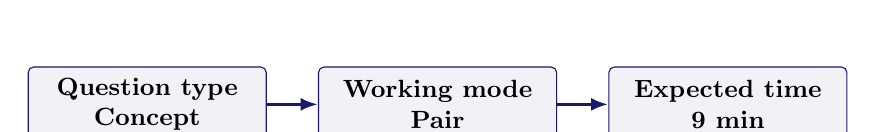
\begin{tikzpicture}[
node distance=0.65cm,
box/.style={draw=MidnightBlue, rounded corners=2pt, minimum height=0.95cm, align=center, font=\small\bfseries, fill=MidnightBlue!6, text width=0.23\linewidth},
arrow/.style={-{Latex[length=2.2mm]}, very thick, MidnightBlue}
]
\node[box] (type) {Question type\\Concept};
\node[box, right=of type] (mode) {Working mode\\Pair};
\node[box, right=of mode] (time) {Expected time\\9 min};
\draw[arrow] (type) -- (mode);
\draw[arrow] (mode) -- (time);
\end{tikzpicture}
\end{center}

{\large\bfseries\color{MidnightBlue} Prompt}\par\medskip
Match these four graph roles to a modern AI system and give one example for each: retrieval for RAG, long-term memory, explanation trace, and multimodal grounding.

{\large\bfseries\color{MidnightBlue} Task details}\par\medskip
\begin{itemize}\item \textbf{Type:} concept
\item \textbf{Mode:} pair
\item \textbf{Time:} 9 min
\item \textbf{Deliverable:} role-to-example mapping
\item \textbf{Assessment focus:} connect graph roles to practical modern AI uses
\item \textbf{Expected length:} 4 rows\end{itemize}

{\large\bfseries\color{MidnightBlue} How to submit}\par\medskip
Post one pair Padlet comment as a four-row list or mini table.

{\large\bfseries\color{MidnightBlue} Discussion in class}\par\medskip
Which role would be easiest to remove, and what would break first?

{\large\bfseries\color{MidnightBlue} Why this helps}\par\medskip
Useful for short questions about what a knowledge graph adds to a modern AI pipeline.

{\large\bfseries\color{MidnightBlue} References}\par\medskip
\begin{itemize}\item Russell \& Norvig (2021) AIMA 4e, Ch.10, pp.314-343
\item Poole \& Mackworth (2023) 3e, Ch.16-17, pp.701-766
\item doi:10.1016/j.cosrev.2026.100902\end{itemize}
\end{tcolorbox}

\begin{tcolorbox}[colback=white,colframe=MidnightBlue,title={Q2 Structured Problem},fonttitle=\bfseries,breakable]
\begin{center}
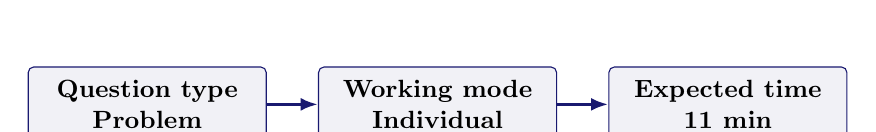
\begin{tikzpicture}[
node distance=0.65cm,
box/.style={draw=MidnightBlue, rounded corners=2pt, minimum height=0.95cm, align=center, font=\small\bfseries, fill=MidnightBlue!6, text width=0.23\linewidth},
arrow/.style={-{Latex[length=2.2mm]}, very thick, MidnightBlue}
]
\node[box] (type) {Question type\\Problem};
\node[box, right=of type] (mode) {Working mode\\Individual};
\node[box, right=of mode] (time) {Expected time\\11 min};
\draw[arrow] (type) -- (mode);
\draw[arrow] (mode) -- (time);
\end{tikzpicture}
\end{center}

{\large\bfseries\color{MidnightBlue} Prompt}\par\medskip
Put these Model Context Protocol (MCP) steps in a sensible order: user intent parse, capability discovery, tool selection, tool call, evidence return, response synthesis, audit log. Add one guardrail beside any two steps.

{\large\bfseries\color{MidnightBlue} Task details}\par\medskip
\begin{itemize}\item \textbf{Type:} problem
\item \textbf{Mode:} individual
\item \textbf{Time:} 11 min
\item \textbf{Deliverable:} ordered workflow
\item \textbf{Assessment focus:} order an MCP request flow and attach guardrails
\item \textbf{Expected length:} 7 ordered steps + 2 guardrails\end{itemize}

{\large\bfseries\color{MidnightBlue} How to submit}\par\medskip
Post your own Padlet comment with the ordered list and two short guardrails.

{\large\bfseries\color{MidnightBlue} Discussion in class}\par\medskip
Which step is most dangerous if it is skipped?

{\large\bfseries\color{MidnightBlue} Why this helps}\par\medskip
Direct practice for workflow-ordering questions about protocol reasoning and tool use.

{\large\bfseries\color{MidnightBlue} References}\par\medskip
\begin{itemize}\item Russell \& Norvig (2021) AIMA 4e, Ch.10, pp.314-343
\item Poole \& Mackworth (2023) 3e, Ch.16-17, pp.701-766
\item https://modelcontextprotocol.io/specification/\end{itemize}
\end{tcolorbox}

\begin{tcolorbox}[colback=white,colframe=MidnightBlue,title={Q3 Structured Problem},fonttitle=\bfseries,breakable]
\begin{center}
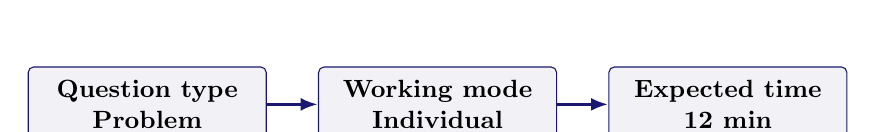
\begin{tikzpicture}[
node distance=0.65cm,
box/.style={draw=MidnightBlue, rounded corners=2pt, minimum height=0.95cm, align=center, font=\small\bfseries, fill=MidnightBlue!6, text width=0.23\linewidth},
arrow/.style={-{Latex[length=2.2mm]}, very thick, MidnightBlue}
]
\node[box] (type) {Question type\\Problem};
\node[box, right=of type] (mode) {Working mode\\Individual};
\node[box, right=of mode] (time) {Expected time\\12 min};
\draw[arrow] (type) -- (mode);
\draw[arrow] (mode) -- (time);
\end{tikzpicture}
\end{center}

{\large\bfseries\color{MidnightBlue} Prompt}\par\medskip
A timetable assistant uses MCP to query a room-change service. Explain the job of each of these four parts in that interaction: the client, the MCP server, the tool or resource being exposed, and the returned evidence.

{\large\bfseries\color{MidnightBlue} Task details}\par\medskip
\begin{itemize}\item \textbf{Type:} problem
\item \textbf{Mode:} individual
\item \textbf{Time:} 12 min
\item \textbf{Deliverable:} role explanation
\item \textbf{Assessment focus:} explain the distinct roles inside a simple MCP interaction
\item \textbf{Expected length:} 4 labelled bullets\end{itemize}

{\large\bfseries\color{MidnightBlue} How to submit}\par\medskip
Post your own Padlet comment with four labelled bullets and one sentence on why this separation helps.

{\large\bfseries\color{MidnightBlue} Discussion in class}\par\medskip
Which role should own access control decisions?

{\large\bfseries\color{MidnightBlue} Why this helps}\par\medskip
Useful for questions that ask students to explain protocol components rather than only list them.

{\large\bfseries\color{MidnightBlue} References}\par\medskip
\begin{itemize}\item Russell \& Norvig (2021) AIMA 4e, Ch.10, pp.314-343
\item Poole \& Mackworth (2023) 3e, Ch.16-17, pp.701-766
\item https://modelcontextprotocol.io/specification/\end{itemize}
\end{tcolorbox}

\begin{tcolorbox}[colback=white,colframe=MidnightBlue,title={Q4 Collaborative Mini-Case},fonttitle=\bfseries,breakable]
\begin{center}
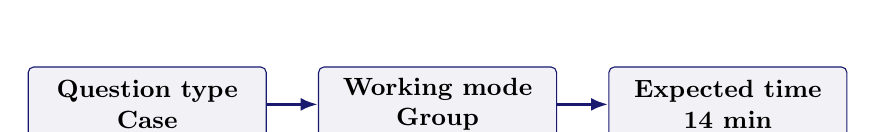
\begin{tikzpicture}[
node distance=0.65cm,
box/.style={draw=MidnightBlue, rounded corners=2pt, minimum height=0.95cm, align=center, font=\small\bfseries, fill=MidnightBlue!6, text width=0.23\linewidth},
arrow/.style={-{Latex[length=2.2mm]}, very thick, MidnightBlue}
]
\node[box] (type) {Question type\\Case};
\node[box, right=of type] (mode) {Working mode\\Group};
\node[box, right=of mode] (time) {Expected time\\14 min};
\draw[arrow] (type) -- (mode);
\draw[arrow] (mode) -- (time);
\end{tikzpicture}
\end{center}

{\large\bfseries\color{MidnightBlue} Prompt}\par\medskip
Design a multi-agent workflow for cybersecurity triage using four roles: detector, correlator, responder, and governance. Include one Agent-to-Agent (A2A) handoff to an external threat-intelligence agent and one trust control before the handoff is accepted.

{\large\bfseries\color{MidnightBlue} Task details}\par\medskip
\begin{itemize}\item \textbf{Type:} case
\item \textbf{Mode:} group
\item \textbf{Time:} 14 min
\item \textbf{Deliverable:} orchestration design
\item \textbf{Assessment focus:} design a multi-agent workflow with one A2A handoff and one governance control
\item \textbf{Expected length:} 4 roles + 1 handoff + 1 control\end{itemize}

{\large\bfseries\color{MidnightBlue} How to submit}\par\medskip
Post one group Padlet comment with the role order, the A2A handoff point, and one governance control.

{\large\bfseries\color{MidnightBlue} Discussion in class}\par\medskip
Which role should be allowed to trigger real action, and which should only advise?

{\large\bfseries\color{MidnightBlue} Why this helps}\par\medskip
Supports case questions on orchestration, handoff, and governance in distributed agent systems.

{\large\bfseries\color{MidnightBlue} References}\par\medskip
\begin{itemize}\item Russell \& Norvig (2021) AIMA 4e, Ch.10, pp.314-343
\item Poole \& Mackworth (2023) 3e, Ch.16-17, pp.701-766
\item https://a2a-protocol.org/dev/\end{itemize}
\end{tcolorbox}

\begin{tcolorbox}[colback=white,colframe=MidnightBlue,title={Q5 Exam-Style Constructed Response},fonttitle=\bfseries,breakable]
\begin{center}
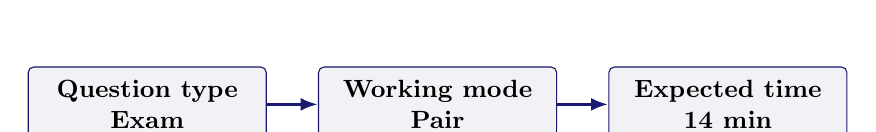
\begin{tikzpicture}[
node distance=0.65cm,
box/.style={draw=MidnightBlue, rounded corners=2pt, minimum height=0.95cm, align=center, font=\small\bfseries, fill=MidnightBlue!6, text width=0.23\linewidth},
arrow/.style={-{Latex[length=2.2mm]}, very thick, MidnightBlue}
]
\node[box] (type) {Question type\\Exam};
\node[box, right=of type] (mode) {Working mode\\Pair};
\node[box, right=of mode] (time) {Expected time\\14 min};
\draw[arrow] (type) -- (mode);
\draw[arrow] (mode) -- (time);
\end{tikzpicture}
\end{center}

{\large\bfseries\color{MidnightBlue} Prompt}\par\medskip
Explain when a knowledge-graph-enhanced pipeline is better than plain text retrieval for a knowledge assistant. Your answer should discuss one strong benefit and one operational risk.

{\large\bfseries\color{MidnightBlue} Task details}\par\medskip
\begin{itemize}\item \textbf{Type:} exam
\item \textbf{Mode:} pair
\item \textbf{Time:} 14 min
\item \textbf{Deliverable:} argument with trade-offs
\item \textbf{Assessment focus:} explain when a KG-enhanced pipeline is better than plain text retrieval and what risk remains
\item \textbf{Expected length:} 180-250 words\end{itemize}

{\large\bfseries\color{MidnightBlue} How to submit}\par\medskip
Post one pair Padlet comment with a clear claim, supporting evidence, and one risk-control idea.

{\large\bfseries\color{MidnightBlue} Discussion in class}\par\medskip
Is the extra graph maintenance worth it for every assistant?

{\large\bfseries\color{MidnightBlue} Why this helps}\par\medskip
Matches exam answers that ask students to weigh architecture benefits against operational costs.

{\large\bfseries\color{MidnightBlue} References}\par\medskip
\begin{itemize}\item Russell \& Norvig (2021) AIMA 4e, Ch.10, pp.314-343
\item Poole \& Mackworth (2023) 3e, Ch.16-17, pp.701-766
\item doi:10.1016/j.cosrev.2026.100902
\item doi:10.1016/j.iswa.2025.200541\end{itemize}
\end{tcolorbox}

\begin{tcolorbox}[colback=white,colframe=MidnightBlue,title={Q6 Stretch Extension},fonttitle=\bfseries,breakable]
\begin{center}
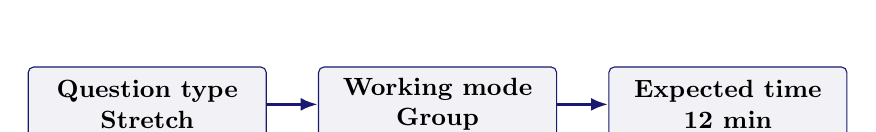
\begin{tikzpicture}[
node distance=0.65cm,
box/.style={draw=MidnightBlue, rounded corners=2pt, minimum height=0.95cm, align=center, font=\small\bfseries, fill=MidnightBlue!6, text width=0.23\linewidth},
arrow/.style={-{Latex[length=2.2mm]}, very thick, MidnightBlue}
]
\node[box] (type) {Question type\\Stretch};
\node[box, right=of type] (mode) {Working mode\\Group};
\node[box, right=of mode] (time) {Expected time\\12 min};
\draw[arrow] (type) -- (mode);
\draw[arrow] (mode) -- (time);
\end{tikzpicture}
\end{center}

{\large\bfseries\color{MidnightBlue} Prompt}\par\medskip
Choose one neuro-symbolic pattern from the lecture - neural-to-symbolic, symbolic-to-neural, or joint constrained reasoning. Propose one concrete use case and explain why that pattern fits better than the other two.

{\large\bfseries\color{MidnightBlue} Task details}\par\medskip
\begin{itemize}\item \textbf{Type:} stretch
\item \textbf{Mode:} group
\item \textbf{Time:} 12 min
\item \textbf{Deliverable:} use-case proposal
\item \textbf{Assessment focus:} choose a neuro-symbolic pattern and justify a realistic application
\item \textbf{Expected length:} 4 bullets\end{itemize}

{\large\bfseries\color{MidnightBlue} How to submit}\par\medskip
Post one group Padlet comment naming the pattern, the use case, and two reasons for the fit.

{\large\bfseries\color{MidnightBlue} Discussion in class}\par\medskip
Which pattern is easiest to explain to a non-technical manager?

{\large\bfseries\color{MidnightBlue} Why this helps}\par\medskip
Good extension for synthesis questions on combining symbolic structure with learned models.

{\large\bfseries\color{MidnightBlue} References}\par\medskip
\begin{itemize}\item Russell \& Norvig (2021) AIMA 4e, Ch.10, pp.314-343
\item Poole \& Mackworth (2023) 3e, Ch.16-17, pp.701-766
\item doi:10.1109/TNNLS.2024.3420218
\item doi:10.1016/j.iswa.2025.200541\end{itemize}
\end{tcolorbox}

\section*{Submission Instructions}

Use the seeded Padlet posts for Q1--Q6. Q2 and Q3 are individual. Q1 and Q5 are pair tasks. Q4 and Q6 should be one joint group comment. Start each comment with your names or group label.

\section*{Whole-Class Debrief Prompts}

\begin{itemize}
\tightlist
\item
  Which part of the MCP flow most clearly needs a guardrail?
\item
  What makes an A2A handoff trustworthy instead of dangerous?
\item
  When is a graph-enhanced pipeline worth the extra maintenance cost?
\end{itemize}

\section*{Exam Transfer Note (Day-Level)}

Maps to exam questions on graph roles in modern AI, MCP flow, protocol roles, multi-agent orchestration, A2A handoff, and architecture trade-offs.

\end{document}
